
\documentclass[12pt,a4paper]{report}

%\RequirePackage[margin=3.0cm,a4paper]{geometry}

\usepackage{amsmath,amssymb,amstext}
\usepackage{times}
\usepackage[T1]{fontenc} 
\usepackage[utf8]{inputenc} 
\usepackage[ngerman]{babel}
\usepackage{graphicx, xcolor} 
\usepackage[
        plainpages=false,
        pdfpagelayout=TwoPageRight,
        pdfborder={0 0 0},
        hyperfootnotes=false
    ]{hyperref}
\usepackage{setspace} %mit /onehalfspacing wird im Textein 1,5 facher Zeilenabstand verwendet
\usepackage{accents}
\usepackage{color, colortbl}

\parindent 0pt


\begin{document}
    \onehalfspacing
    
    \begin{titlepage}
        \centering
        
\includegraphics[width=0.4\textwidth]{./LogoSoFar.png}\par\vspace{1cm}
        {\scshape \LARGE BWolf \\ \Large Eine webbasierte Plattform zur
            Einschreibung und Verwaltung des
            Empiriepraktikums an der FSU Jena\par}
        \vspace{1.5cm}
        {\huge\bfseries Dokumentation\par}
        \vspace{1.5cm}
        {\large\itshape Christoph Keiner, Matthias Reuse, Ingo Schäfer, Christoph Staudt\par}
        \vspace{1.0cm}
        {\large \today\par}
    \end{titlepage}

    \pagenumbering{Roman}  
    \section*{Eigenständigkeitserklärung}
        Wir erklären, dass wir die vorliegende Arbeit selbstständig und nur unter Verwendung der angegebenen Quellen und Hilfsmittel angefertigt haben.\\\\\\
        Jena, \today\\
        
        \begin{figure}[h]
            \begin{tabular}{@{}c@{}}
                % Unterschrift Fred    
            \end{tabular}
            \hspace{.01\textwidth}
            \begin{tabular}{@{}c@{}}
                \includegraphics[width=.23\textwidth]{./UnterschriftMatthias.png}
            \end{tabular}
            \hspace{.01\textwidth}
            \begin{tabular}{@{}c@{}}
                % Unterschrift Ingo
            \end{tabular}
            \hspace{.01\textwidth}
            \begin{tabular}{@{}c@{}}
                \includegraphics[width=.23\textwidth]{./UnterschriftChristoph.jpg}
            \end{tabular}
        \end{figure}
        \thispagestyle{empty}
        \pagebreak
        
    \tableofcontents 
    \clearpage
    \pagenumbering{arabic}
    
    
    \chapter{Einleitung}
\label{chapter:introduction}

    \section{Motivation}
    \label{sec:motivation}
        Jedes Jahr wird an der Friedrich-Schiller-Universität Jena das Empiriepraktikum vom Institut für Psychologie angeboten.
        Dabei handelt es sich um eine Pflichtveranstaltung, die jeder Psychologie-Student absolviert haben muss.
        Innerhalb eines Praktikums werden mehrere Kurse angeboten.
        An einem dieser Kurse muss der Studierende teilnehmen, um das Modul erfolgreich abzuschließen.
        Allerdings ist die Teilnehmerzahl eines jeden Kurses begrenzt.
        So kann nicht jeder der über einhundert Studenten zu seinem Wunschkurs zugelassen werden.
        Die naheliegende Lösung ist die Zuweisung zu den Kursen nach Geschwindigkeit der Studenten bei der Anmeldung.
        Allerdings ist diese Verteilungsstrategie mit viel Stress und Streit verbunden.
        Die Studenten müssen anders auf die Kurse verteilt werden.
        Hierzu dient dem Institut für Psychologie eine Zuweisung zu den Kursen mittels Präferenzlisten.
        Jeder Studierende erstellt eine Liste mit Präferenzen, wie gerne er an welchen Kurs teilnehmen möchte.
        Es liegt auf der Hand, dass diese Listen nun nicht alle per Hand ausgewertet werden können, sondern automatisch erfolgen muss.
        Für diese Aufgabe existieren bereits Lösungen.
        So können mit dem Studienverwaltungstool der FSU Jena Friedolin Studenten bereits Präferenzlisten erstellt und ausgewertet werden.
        Bei der Verteilung mithilfe von Friedolin kommt es jedoch zu Problemen, da beim Erstellen der Präferenzliste getrickst werden kann.
        Aus diesem Grund hat das Institut für Psychologie bereits eine eigene Plattform geschaffen, die das aufnehmen der Präferenzliste und das Verteilen auf die Kurse übernimmt.
        Hierbei ist aber die Verteilung auf die verschiedenen Kurse oft nicht zufriedenstellend und es muss manuell das Ergebnis angepasst werden.
        Das mit dieser Arbeit verbundene Projekt beschäftigt sich nun mit dem Erstellen einer neuen Plattform für das Empiriepraktikum und der Frage, wie sich die Studenten besser auf die Kurse verteilen lassen.
        
    \section{Aufgabenstellung}
    \label{sec:task}
        Es gilt eine webbasierte Plattform für die Verwaltung des Empiriepraktikums der FSU Jena zu erstellen.
        Hauptaufgabe dieser Plattform ist, den verantwortlichen Mitarbeitern des Instituts für Psychologie zu ermöglichen, für ein kommendes Semester ein neues Praktiumsmodul mit allen zugehörigen Kursen anlegen zu können.
        Des Weiteren sollen die Studenten die Möglichkeit erhalten eine Präferenzliste zu erstellen, welche der angebotenen Kurse sie am liebsten besuchen möchten.
        Nach Ablauf einer vorher festzulegenden Frist sollen die Studenten gemäß ihrer Präferenzliste dann automatisch bestmöglich auf die Kurse verteilt werden.
        Hierzu soll ein geeigneter Verteilungsalgorithmus entwickelt werden.


    \section{Aufbau der Arbeit}
    \label{sec:structure}
       Zunächst werden in dieser Arbeit die Anforderungen an die Plattform, sowie den Verteilungsalgorithmus ausgehend von der Aufgabenstellung aus Abschnitt \ref{sec:task} näher spezifiziert.
       Anschließend wird der Entwurf für die Realisierung der Anforderungen an das zu entwickelnde System dargestellt.
       Danach folgt eine Beschreibung der tatsächlichen Umsetzung des Systems.
       Im Anschluss wird der Algorithmus zur Verteilung der Studenten formal beschrieben.
       Hiernach werden die durchgeführten Tests zu Plattform und Verteilungsalgorithmus vorgestellt.
       Abschließend wird die Arbeit nochmals kurz zusammengefasst und ein Ausblick auf weitere umzusetzende Funktionalitäten gegeben.
       
    \chapter{Anforderungsanalyse}
    \section{Allgemeine Problemstellung}
    \label{Problemstellung}
        Im Zuge des Projektes gilt es eine webbasierte Plattform zu schaffen, die die Verwaltung des Empiriepraktikums der FSU Jena ermöglicht.
        Hauptaufgabe dieser Plattform ist, den verantwortliche Mitarbeitern der FSU Jena zu ermöglichen, für ein kommendes Semester ein neues Praktiumsmodul mit allen zugehörigen Kursen anlegen zu können.
        Des Weiteren sollen die Studenten die Möglichkeit erhalten eine Präferenzliste zu erstellen, welche der angebotenen Kurse sie am liebsten besuchen möchten.
        Nach Ablauf einer vorher festzulegenden Frist sollen die Studenten gemäß ihrer Präferenzliste dann automatisch bestmöglich auf die Kurse verteilt werden.     
    
    \section{Genaue Anforderungen an das System}
        Gemäß der allgemeinen Problemstellung aus Abschnitt \ref{Problemstellung} existieren verschiedene Sichtweisen auf die Anforderungen des Systems.
        Zum einen die Sicht der Verantwortlichen für Praktikum und Kurse, zum anderen die der Studenten.
        Erstere teilt sich wiederum auf in den Blickwinkel der Dozenten der einzelnen Kurse und der übergeordneten Verantwortlichen für das Empiriepraktikum, im Weiteren Administratoren genannt.
        Im Folgenden werden zunächst die Anforderungen für Studenten, Dozenten und Administratoren anhand des chronologischen Ablaufs eines Praktikumsmoduls dargestellt.
        Anschließend wird nochmal für die jeweiligen Sichten eine kurze Übersicht gegeben, sowie weitere detailliertere Anforderungen genannt.
        
        \subsection{Ablauf eines Praktikumsmoduls}
            Der Ablauf beginnt, indem die Administratoren, nachdem sie sich in einer Login-Oberfläche angemeldet haben, ein neues Praktikumsmodul erstellen.
            Zu diesem Praktikumsmodul gehören neben generellen Informationen wie Name und Semester auch die besonderen Angaben, ab wann Studenten ihre Präferenzliste erstellen können und zu welchem Zeitpunkt die automatische Verteilung vorgenommen werden soll.
            Im Anschluss können die Dozenten, nachdem auch sie sich in einer entsprechenden Oberfläche angemeldet haben, ihre Kurse zu dem aktuellen Praktikumsmodul hinzufügen.
            Dabei sollen Kurse Angaben über Titel, Dozent, Teilnehmerzahl, Ort, Zeit, Beschreibung des Kurses und eine Literaturliste besitzen.
            Zusätzlich soll ein Kurs Informationen über den Lehrstuhl, sowie die Finanzierung erhalten, die jedoch nicht für Studenten einsehbar sein soll.
            Nachdem alle Dozenten ihre Kurse eingetragen haben, sollen die Administratoren die aktuelle Kursübersicht online stellen können, sodass jeder die Kurse einsehen kann.
            Besteht Interesse, dass Empiriepraktikum in diesem Semester zu absolvieren, so sollen sich die Studierenden registrieren können.
            Nach der Registrierung können die Studenten ihre Präferenzliste erstellen und speichern.
            Dabei soll die soll Präferenzliste auch jederzeit vom Studierenden noch verändert werden können.
            Nach jeder gespeicherten Änderung soll der Student eine Email-Benachrichtigung mit seiner aktuellen Präferenzliste erhalten.
            Nach Ablauf der zuvor von den Administratoren festgelegten Frist sollen die Studenten automatisch anhand ihrer aktuellen Version der Präferenzliste auf die Kurse verteilt werden.
            Diese Verteilung sollte möglichst gut sein, d.h. in Fall dieses Projekts eine möglichst gleichmäßige Verteilung der Studenten mit wenigen Ausreißern nach Unten.
            Nach dieser automatischen Verteilung soll eine Nachbearbeitungsphase folgen, in der die Administratoren den Algorithmus bei Bedarf mit vielleicht anderen Parametern neu starten können.
            Es soll jedoch auch die Möglichkeit geben, das Ergebnis der Verteilung manuell zu ändern.
            Nachdem das Ergebnis der Verteilung feststeht, sollen alle Beteiligten Studenten und Dozenten über das Ergebnis der Verteilung mittels einer Email-Benachrichtigung informiert werden.
            Ab diesem Moment sollen die Teilnehmer jedes Kurses für jeden sichtbar sein.
            \textcolor{red}{Erwähnung der Tauschperiode? Nur für den Fall, dass wir sie wirklich am Ende implementieren}
            
            
                    
        \subsection{Verschiedene Sichten im Überblick}
        \label{Sichten}
            \subsubsection{Sicht der Administratoren}
                Administratoren haben die Möglichkeit ein neues Praktikum zu erstellen.
                Dabei müssen sie Angaben über Name, Semester, Frist für die Anmeldung und Beginn der automatischen Verteilung festlegen.
                Sie sollen aktiv die Kursübersicht für das aktuelle Praktikum veröffentlichen können.
                Des Weiteren können Administratoren den Verteilungsalgorithmus in der Nachbearbeitungsphase erneut mit anderen Parametern starten und die Verteilungsergebnisse auch manuell verändern.
                Zusätzlich sollen Administratoren die angemeldeten Dozenten verwalten können, um z.B. Dozenten, die keine Kurse mehr anbieten zu entfernen.
                Auch sollen die Administratoren Kurse als \glqq freibleiben\grqq markieren können, sowie die maximale und minimale Teilnehmerzahl für alle Kurse fließend einstellen können, falls nötig.
                Die Administratoren sollen für Praktikum auch die Möglichkeit erhalten Filterfunktionen anzuwenden und sich so z.B. die Kurse nach Lehrstühlen sortiert anzeigen zu lassen.
    
            \subsubsection{Sicht der Dozenten}
                Ein Dozent hat die Möglichkeit, Kurse für das aktuelle Praktikum zu erstellen und sich seine Kurse für ältere Praktika nochmals anzusehen, um sie evtl. als Vorlage für neue Kurse zu nutzen. 
                Für einen Kurs müssen sie folgendes angeben:
                \begin{itemize}
                    \item Name
                    \item Titel
                    \item Dozenten
                    \item Zeit/Raum
                    % Minimale Teilnehmer fällt raus, da die Psychologen festegelegt haben, es müssen mindestens 3 Leute in jedem Kurs sein
                    \item Teilnehmerzahl, hierbei können Dozenten nur zwischen 5 oder 10 wählen
                    \item Kurzbeschreibung
                    \item Beschreibung
                    \item Literatur
                    \item E-Mail Adresse des Empirie-Praktikums-Leiter %? Ist das nicht nur die vom Dozenten
                \end{itemize}
                Folgendes ist nicht für den Studenten einsehbar:
                \begin{itemize}
                    \item Lehrstuhl
                    \item Lehrauftrag
                    \item \textcolor{red}{Erstes Mal Empiriepraktikum?}
                \end{itemize}
                Der Inhalt von längeren Angaben wie der Beschreibung des Praktikums, soll in einer Textumgebung möglich sein, in der geeignete Textformatierung möglich ist.
                Außerdem sollen auch Bilder in die Beschreibung eingearbeitet werden können.
                Des Weiteren sollen Dozenten nur ihre eigenen Kurse editieren können.
                Nachdem die Studenten verteilt worden sind, sollen die Dozenten eine E-Mail mit den Studenten, die in ihrem Kurs sind, erhalten.
                \textcolor{red}{Im Verlaufe des Semesters können Dozenten ihren Kurs in zwei Kurse aufteilen.}
    
                
            \subsubsection{Sicht der Studenten}
                Die Studenten sollen ohne eine Registrierung die Kursübersicht aufrufen können, sobald die Administratoren die Kursübersicht veröffentlicht haben.
                Nach der Registrierung sollen die Studenten bis zu einer Frist eine Präferenzliste erstellen und späterhin auch bearbeiten können.
                Bei jeder angenommenen Änderung der Präferenzliste soll ein Studierenden über seine aktuelle Wahl per Email informiert werden.
                Nachdem die Verteilung vom Algorithmus vorgenommen wurde, sollen die Studenten über ihr Ergebnis informiert werden, sowie die Ergebnisse der gesamten Verteilung einsehen können.
    %		 Tauschphase vor eigentlichem Beginn der Veranstaltung mit Email an die Dozenten & Administratoren
    
    
    %	Das ganze offen und Modular halten für andere Module als das Empiriepraktikum
    %	Dabei auf Hierarchie von Präferenzen achten
    %	evtl. die Möglichkeit falls mehr Studenten als Kurse, neue Kurse hinzufügen können
    %	evtl. ein Archiv
    
    
            
    
    \section{Der Verteilungsalgorithmus}
    Der Verteilungsalgorithmus verteilt alle Studenten auf die Kurse.
    Dabei ist es wichtig, dass die aufaddierte maximale Teilnehmeranzahl der Kurse größer ist als die Anzahl der zu verteilenden Studenten.
    Sollte dem nicht der Fall sein, so wird der Administrator informiert.
    Dieser hat dann die Möglichkeit die maximale Teilnehmeranzahl von Kursen zu erhöhen.
    Die Eingabe des Algorithmus sind die Gewichte der Präferenzen und (optional) die Auswahl eines Optimierungsalgorithmus.
    
    Startet der Algorithmus, so versucht er, für jeden Studenten die größte, mögliche Präferenz zu den Kursen zu wählen.
    Dabei ist insbesonders wichtig, dass die Streuung der gewählten Präferenzen möglichst gering ist.
    Dies erfolgt beispielsweise durch eine Gewichtung der Präferenzen.\\
    Weiterhin platziert der Algortihmus in jeden Kurs mindestens drei Studenten, damit der Kurs sinnvoll angeboten werden kann.
    Es werden aber nie mehr Teilnehmer einem Kurs zugeordnet als die maximale Teilnehmeranzahl des Kurses vorgibt.
    
    Hat der Algorithmus schließlich eine passende Zuordnung von Studenten zu Kursen gefunden, so wird der Administrator zuerst benachrichtigt.
    Dieser kann die Ergebnisse bearbeiten, Parameter des Algorithmus neu einstellen, Kurse aktivieren/deaktivieren und ihn erneut starten.
    Ist der Administrator zufrieden mit der Verteilung, so bestätigt dieser das Ergebnis.
    Anschließend wird an die Dozenten eine E-Mail mit ihren Teilnehmern geschickt, und Studenten erhalten eine E-Mail mit ihrem Kurs.
    %    \item Nach Ende der Einschreibung, startet der Algortihmus automatisch. -> unsicher ob sie es so wollten durch die verschiedenen Einstell-Möglichkeiten. Sie hatten im Gespräch beides gesagt.
    
    \section{Technische Details}
    Der Login wird über eine E-Mail/Passwort Authentifizierung realisiert.
    Dafür werden nur E-Mail Adressen der FSU Jena nutzbar sein. Dies bedeutet, dass E-Mails auf ''@uni-jena.de''enden müssen.
    Man kann sich zu jeder Zeit ein- und ausloggen.\newline
    
    Bei der Wahl der Präferenzen darf keine Präferenz doppelt belegt werden, d.h. jede Präferenz hat einen eindeutigen Kurs. \newline %egal option?
    
    Der Verteilungsalgorithmus kann mit verschiedenen Optionen angesteuert werden. Optionen können u.a. die Gewichtung der Varianz, oder welche Kurse belegt werden können, sein. Weiterhin ist der Verteilungsalgorithmus innerhalb von 24 Stunden fertig. \newline
    
    
    \begin{itemize}
    \item Man kann sich zu einem beliebigen Zeitpunkt einloggen und ausloggen.
    \item Der Verteilungsalgorithmus braucht maximal 24 Stunden.
    \item Die Website muss auch auf mobilen Endgeräten funktionieren.
    \item Sollte ein Browser älter als IE11 sein, so wird den Nutzer angezeigt, dass sie ihren Browser updaten sollen.
    \item Die Website wird auf einer docker-compose Umgebung aufgesetzt.
    \item Die Website wird mit OctoberCMS mit Laravel 5.5 umgesetzt.
    \item Der Webserver wird mit Nginx umgesetzt.
    \item Die Datenbank wird mit MySQL umgesetzt.
    \item Der Cache-Server wird mit Redis umgesetzt.
    \item Tests erfolgen für die wesentlichsten Bestandteile, insbesondere für den Algorithmus.
    \item Kursinformationen sind öffentlich einsehbar.
    \item Kurse können von nicht-Studenten insbesondere nach folgenden Kriterien gefiltert werden: 
        \begin{itemize}
        \item Lehrstuhl
        \item Finanzierung/Lehrauftrag
        \item Erstes Mal Empiriepraktikum?
        \end{itemize}
    \end{itemize}

    \definecolor{red}{rgb}{0.827,0.196,0.122}
\definecolor{orange}{rgb}{1.0,0.498,0.0}
\definecolor{olive}{rgb}{0.71,0.71,0.345}
\definecolor{green}{rgb}{0.118,0.490,0.216}
\definecolor{blue}{rgb}{0.447,0.624,0.812}

\chapter{Entwurf}
\label{chapter:design}
    Nachdem im vorangegangenem Kapitel die Anforderungen für das System spezifiziert wurden, soll in diesem Kapitel der Umsetzungsentwurf der verschiedenen Sichten dargestellt werden.
    Zunächst wird das dem System zugrundeliegende Datenmodell dargestellt.
    Darauffolgend wird das Design für die webbasierte Plattform erläutert.     
    
    \section{Datenmodell}
        \begin{figure}
            \centering
            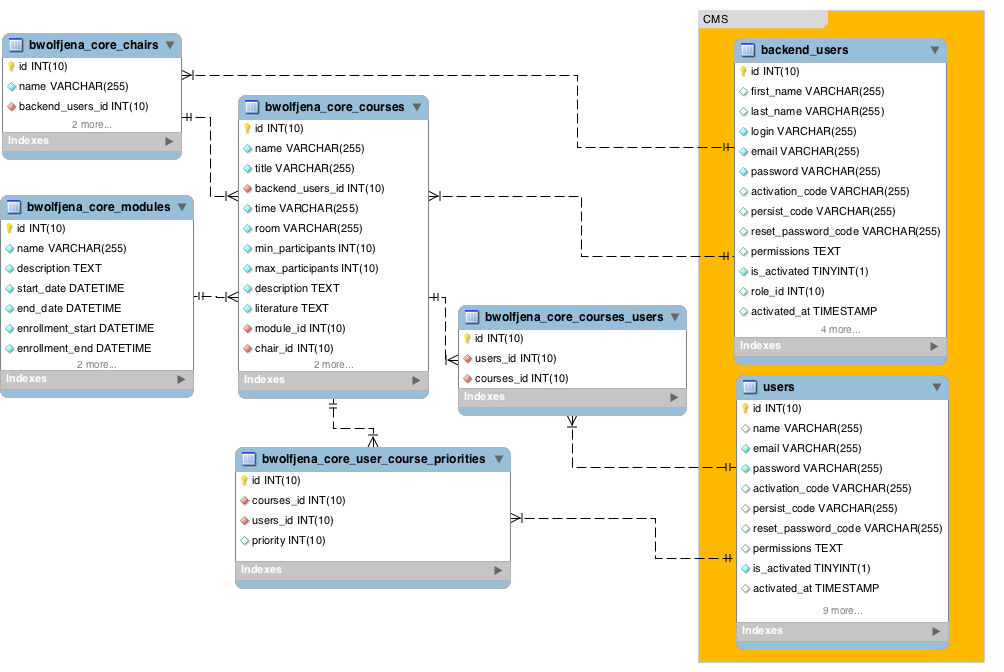
\includegraphics[width=1.0\textwidth]{./design/images/data-model.png}\par\vspace{1cm}
            \caption{Entwurf des Datenmodells. Farbcode für Spalten der Tabellen: Gelb Primärschlüssel, Rot Fremdschlüssel, Blau gewöhnliche Variable, Weiß nullable Variable}
            \label{fig:datamodel}
        \end{figure}
    
        Der Entwurf für das Datenmodell ist in Abbildung \ref{fig:datamodel} zu sehen.
        Es besteht aus sieben Tabellen.
        Die Tabelle \textit{bwolfjena\_core\_modules} beinhaltet die verschiedenen Empiriepraktika.
        Der Name Module für die Tabelle wurde gewählt, da das System bei Bedarf auch auf andere ausgewählte Module als das Empiriepraktikum erweitert werden kann.
        
        In der Tabelle \textit{bwolfjena\_core\_courses} sind die verschiedenen Kurse gespeichert.
        Ein Kurs gehört immer zu einem bestimmten Modul beziehungsweise einem Empiriepraktikum.
        Um das abzubilden, ist für jeden Kurs mittels eines Fremdschlüssels das Empiriepraktikum, zu dem er gehört, gespeichert.
        
        Ein Kurs wird immer von einem Lehrstuhl angeboten, die in der Tabelle \textit{bwolfjena\_core\_chairs} abgelegt sind.
        Auch auf diese Tabelle existiert wieder ein entsprechender Fremdschlüssel in \textit{bwolfjena\_core\_courses}. 
        
        Alle angemeldeten Studenten werden in der Tabelle \textit{users} gespeichert.
        Jeder der Studenten hat eine Präferenzliste.
        Die Einträge der Präferenzliste für jeden Studenten und jeden Kurs werden in Tabelle \textit{bwolfjena\_core\_priorities} gespeichert.
        Dementsprechend beinhaltet \textit{bwolfjena\_core\_priorities} Fremdschlüssel von \textit{users} und \textit{bwolfjena\_core\_courses}.
        
        In der Tabelle \textit{bwolfjena\_core\_users} ist abgelegt, welcher Student welchem Kurs zu geteilt wurde.
        Aus diesem Grund beinhaltet \textit{bwolfjena\_core\_users} Fremdschlüssel auf \textit{bwolfjena\_core\_courses} und \textit{users}. 
        
        Die letzte Tabelle \textit{backend\_users} beinhaltet die Backendbenutzer.
        Damit sind die Dozenten und Administratoren gemeint.
        In \textit{bwolfjena\_core\_courses} ist ein Fremdschlüssel für die Backendbenutzer gespeichert, um den Dozenten anzugeben, der den Kurs leitet.
        Auch die Tabelle \textit{bwolfjena\_core\_chairs} hat einen Fremdschlüssel zu der Tabelle \textit{backend\_users}, um den Lehrstuhlinhaber anzugeben.
        
        Neben den beschriebenen Fremdschlüsseln existieren für die Einträge in jeder Tabelle IDs als Primärschlüssel.
        Die weiteren Spalten der Tabellen sind entsprechend den Anforderung aus Kapitel \ref{chapter:requirements} gewählt.
        
        
        
    
    \section{Design}
        Für den Desing-Entwurf der Seite wurden Mock-Ups erstellt, die den groben Aufbau der Website mit den entsprechenden Funktionen zeigen. 
        Im folgenden werden diese Mock-Ups für das sogenannte Frontend, also aus Sicht der Studenten, und für das Backend, die Sicht der Dozenten beziehungsweise der Administratoren, vorgestellt.
        Dabei gilt der in Tabelle \ref{tab:Farbcode} angegebene Farbcode für die verschiedenen Elemente der Mock-Ups.
        \begin{table}
            \centering
            \begin{tabular}{l c| l}
                \cellcolor{red} & & Eingabefeld\\
                \cellcolor{orange} & & Button\\
                \cellcolor{olive} & & Drag\&Drop-Element\\
                \cellcolor{green} & & Textfeld\\
                \cellcolor{blue} & & Optisches Element
            \end{tabular}
            \caption{Farbcode der Mockups}
            \label{tab:Farbcode}
        \end{table}
    
        \subsection{Frontend}
            Wie in Kapitel \ref{chapter:requirements} bereits ausgeführt, sollen die Studenten zunächst eine Registrierungs- bzw. Login-Oberfläche sehen.
            Jedoch sollen die verschiedenen Kurse auch ohne eine Anmeldung einsehbar sein.
            \begin{figure}[t]
            	\centering
            	\includegraphics[width=0.6\textwidth]{./design/images/MockUpsFrontend/frontendLogin.png}
            	\caption{Entwurf für die Login-Oberfläche}
            	\label{fig:mockupLoginFrontend}
            \end{figure}   
        
            In Abbildung \ref{fig:mockupLoginFrontend} werden beide Anforderungen umgesetzt.
            Zum einen die Login-Oberfläche, in der in zwei Textfeldern Benutzername und Passwort für einen erfolgreichen Login eingetragen werden müssen, zum anderen die direkte Weiterleitung zur Kursübersicht als einfacher Knopf darunter.

            Die Kopfzeile umfasst einige Reiter.
            So kann mithilfe der Kopfzeile auf die verschiedenen Funktionen des Frontends gewechselt werden. 
            Dazu zählen die Kursübersicht, die Erstellung der Präferenzliste, das Einsehen der Verteilungsergebnisse, sowie das Tauschen von Kursen.
            Außer der Navigation auf die Kursübersicht sind diese jedoch erst nach einer erfolgreiche Anmeldung funktional.
            Ohne eine Anmeldung wird der Benutzer wieder auf die Login-Oberfläche verwiesen.
            In der Kopfzeile soll auch eine Schaltfläche zum erstmaligen Registrieren im System sein.
            Die Registrierungsseite gleicht strukturell der Login-Oberfläche aussehen.
            Sobald ein Benutzer sich erfolgreich angemeldet hat, soll der Schalter zum Anmelden in der Kopfzeile gegen einen Abmelden-Knopf ausgetauscht werden.
%            Auch eine Anzeige, ab wann das Ende der Einschreibungs- und Tauschphase erreicht ist.
			Auf allen weiteren Seiten des Frontends soll die Kopfzeile die gleichen Funktionen und das gleiche Aussehen haben, der Registieren-Knopf entfällt jedoch, sobald die Anmeldung erfolgt ist.
            Die Fußzeile soll weitere allgemeine Informationen bereitstellen, sofern diese von Nöten sein sollten, aber vor allem als optischer Abschluss der Seite dienen.
            Auch sie soll auf alle folgenden Seiten übernommen werden.
			
			\begin{figure}[t]
				\centering
				\includegraphics[width=0.6\textwidth]{./design/images/MockUpsFrontend/frontendCourses.png}
				\caption{Entwurf für die Kursübersicht}
				\label{fig:mockupCoursesFrontend}
			\end{figure}
			
			In Abbildung \ref{fig:mockupCoursesFrontend} ist die Seite für die Kursübersicht zu sehen.
            Unter der Kopfzeile folgt eine textuelle Erklärung des Ablaufs des Empiriepraktikums und der für die Studenten relevanten Schritte, um sich erfolgreich für die Kurse einzuschreiben.
            Die verschiedenen Kurse werden darunter jeweils mit einer kurzen Beschreibung angezeigt.
            Durch einen Klick auf ein Kursfeld, sollen sich die detaillierten Informationen zu dem Kurs einsehen lassen.
            Das Design hierfür ist in Abbildung \ref{fig:mockupDetailsFrontend} zu sehen und bedarf keiner weiteren Erläuterung.
            
            \begin{figure}[t]
            	\centering
            	\includegraphics[width=0.6\textwidth]{./design/images/MockUpsFrontend/frontendPreferences.png}
            	\caption{Entwurf für die Einschreibungs-Oberfläche}
            	\label{fig:mockupPreferencesFrontend}
            \end{figure}
            
            Die Seite für die Einschreibung in die Kurse soll wie in Abbildung \ref{fig:mockupPreferencesFrontend} gestaltet sein.
            Wieder bilden Kopfzeile und Fußzeile den Rahmen der Seite.
            Unter der Kopfzeile befindet sich auch hier eine kurze Erklärung, wie man die Präferenzliste genau erstellt.
            Das Erstellen soll im Feld \textit{Präferenzliste} über ein ''Drag\&Drop''-System vorgenommen werden und über den Knopf \textit{Absenden} fixiert werden können.
            
            Nachdem die Verteilung auf die Kurse vorgenommen wurde, sollen die Benutzer unter dem Reiter Ergebnisübersicht die Resultate einsehen können.
            Der Entwurf hierfür gleicht dem für die Kursübersicht.
            Statt einer Beschreibung des Kurses, werden allerdings die Teilnehmer der Kurse angezeigt.
            
            Unter dem Reiter \textit{Tauschbörse} soll die in Kapitel \ref{chapter:requirements} genannte Tauschmöglichkeit für Studenten realisiert sein.
            Die Struktur der Seite gleicht dem der Kursübersicht.
            Unter einer Information in welchem Kurs man sich befindet und wie die Tauschfunktionen zu benutzten sind, finden sich die verschiedenen Kurse, genauso wie in der Kursübersicht.
            Der Kurs, dem man zugeteilt ist, erscheint ausgegraut oder auf eine andere Art und Weise markiert.
            
            \begin{figure}[t]
            	\centering
            	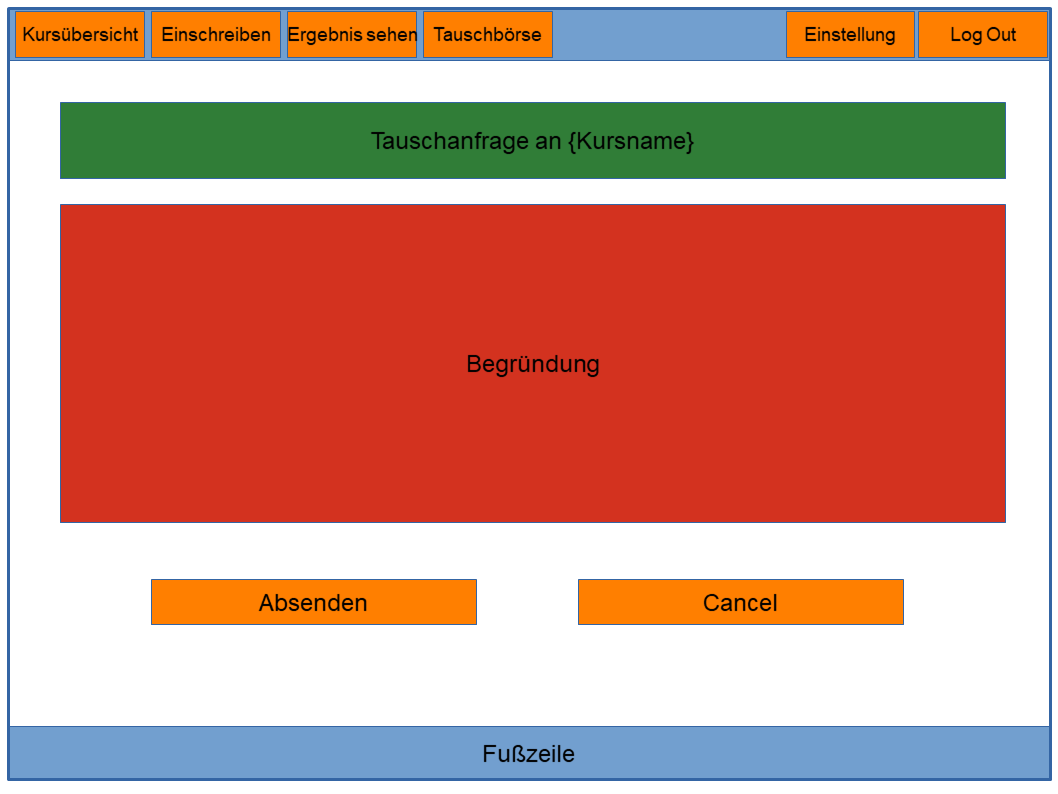
\includegraphics[width=0.6\textwidth]{./design/images/MockUpsFrontend/frontendSwap2.png}
            	\caption{Entwurf für die Tauschanfrage}
            	\label{fig:mockupResultsSwap2}
            \end{figure}
            
            Durch einen Klick auf den Kurs mit dem man Tauschen möchte, öffnet sich die in Abbildung \ref{fig:mockupResultsSwap2} gezeigt Seite.
            Hier kann in dem Textfeld \textit{Begründung} eine Begründung für den Tausch angegeben werden.
            Mit der Schaltfläche \textit{Absenden} kann die Tauschanfrage abgeschickt werden, mit \textit{Abbrechen} gelangt der Benutzer wieder auf die vorherige Ansicht der Tauschbörse.
            
            
            
        
            
            
    
        \subsection{Backend}
	        Im Folgenden werden die wichtigsten Mockups für Administratoren und Dozenten vorgestellt.
	        Für beide Sichten gibt es wieder eine Kopf- und eine Fußzeile.
	        Die Kopfzeile für die Administratoren umfasst zunächst einen Reiter \textit{Verwalten}, in dem Kurse, Module und Lehrstühle angelegt werden können.
	        Des Weiteren gibt es den Reiter \textit{Benutzer}, unter dem alle Benutzer des Systems verwaltet werden können.
	        Unter dem Reiter \textit{Verteilung} können die Administratoren den Verteilungsalgorithmus starten und sich die Ergebnisse anzeigen lassen.
	        Zusätzlich gibt es noch eine Seitenleiste, in der unter dem jeweiligen Reiter weitere Optionen zur Verfügung stehen.
        	
        	\begin{figure}[t]
        		\centering
        		\includegraphics[width=0.6\textwidth]{./design/images/MockUpsBackend/backendManageCourses.png}
        		\caption{Entwurf für das Verwalten der Kurse}
        		\label{fig:mockupManageCourses}
        	\end{figure}
        	
        	In Abbildung \ref{fig:mockupManageCourses} ist beispielhaft für den Reiter Verwaltung, die der Kursverwaltung zu sehen.
        	Mithilfe der Seitenleiste am linken Rand, kann zwischen dem Verwalten von Kursen, Modulen (Praktika) und Lehrstühlen gewechselt werden.
        	Alle Vorhandenen Kurse (bzw. Module oder Lehrstühle) werden in einer Tabelle angezeigt.
        	Mit den beiden Schaltflächen am oberen Rand der Tabelle kann ein neuer Eintrag in der jeweiligen Tabelle erstellt, bzw. ein vorhandener Eintrag gelöscht werden.
        	Die Einträge der entsprechenden Tabelle können nachträglich durch einen Klick auf den Eintrag in der Tabelle geändert werden.
        	
            \begin{figure}[t]
                \centering
                \includegraphics[width=0.6\textwidth]{./design/images/MockUpsBackend/backendEdit.png}
                \caption{Entwurf für das editieren eines Kurses}
                \label{fig:mockupEdit}
            \end{figure}
              
        	Abbildung \ref{fig:mockupEdit} zeigt den Entwurf für das Erstellen oder Ändern eines Kurses, Moduls oder Lehrstuhls.
        	Alle notwendigen Informationen sollen in Textfeldern eingegeben und mit geeigneten Textformatierungsoptionen bearbeitet werden können.
        	Mit einen Klick auf die Schaltfläche \textit{Speichern} wird die Änderung übernommen, bzw. die Erstellung bestätigt.\\
        	
        	Die Verwaltung der Benutzer erfolgt auf die selbe Weise und gleicht sich im Design.
        	Wieder kann mithilfe der linken Seitenleiste umgeschaltet werden, ob Studenten oder Dozenten verwaltet werden sollen.
        	Die entsprechende Benutzergruppe werden in einer Tabelle angezeigt und können mittels einer Schaltfläche gelöscht werden.
        	Durch einen Klick auf die Tabellenzeile sollen die Informationen der Benutzer analog zum Bearbeiten der Kurse oder Module  geändert werden können.\\
            
            \begin{figure}[t]
                \centering
                \includegraphics[width=0.6\textwidth]{./design/images/MockUpsBackend/backendDistribution.png}
                \caption{Entwurf für das Anzeigen der Verteilungsvorschläge}
                \label{fig:mockupDistribution}
            \end{figure}
        	
        	Für die Steuerung des Verteilungsalgorithmus unter dem Reiter \textit{Verteilung}, muss zunächst aus einer Liste dass entsprechende Praktikum ausgewählt werden.
            Danach wird die Verteilung für dieses Modul mit verschiedenen Parametern ermittelt und anschließend werden die Ergebnisse mithilfe von geeigneten Grafiken angezeigt.
            Der Entwurf für diese Seite ist in Abbildung \ref{fig:mockupDistribution} zu sehen.
            Durch einen Klick auf den entsprechende Verteilungsvorschlag, soll dieser als Ergebnis übernommen werden.\\
        	
        	Die Ansicht der Dozenten unterscheidet sich lediglich im Funktionsumfang.
        	So sehen die Dozenten nur den Reiter \textit{Verwalten} in der Kopfzeile und in der linken Seitenleiste nur die Option zum verwalten der Kurse.
        	Die Tabelle zeigt jetzt nur die Kurse, die der entsprechende Dozent selbst angelegt hat.  
        	
        	
        	
        	
        	
        	
        	
        	
        	
    \chapter{Umsetzung}
\label{chapter:implementation}
    In diesem Kapitel wird die Umsetzung des System erläutert.
    Zunächst wird die zur Implementierung verwendete Software näher erläutert.
    Anschließend werden Front- und Backend kurz vorgestellt und mit dem Entwurf aus Kapitel \ref{chapter:design} verglichen.
    
    \section{Verwendete Software}
        
    
    \section{Frontend}
        Die Entwürfe für das Frontend wurden ohne große Änderungen umgesetzt.
        
        \begin{figure}
            \centering
            \begin{subfigure}{0.49\textwidth}
                \includegraphics[width=1.0\textwidth]{./implementation/images/MockUpsFrontend/frontendLogin.png}
            \end{subfigure}
            \begin{subfigure}{0.49\textwidth}
                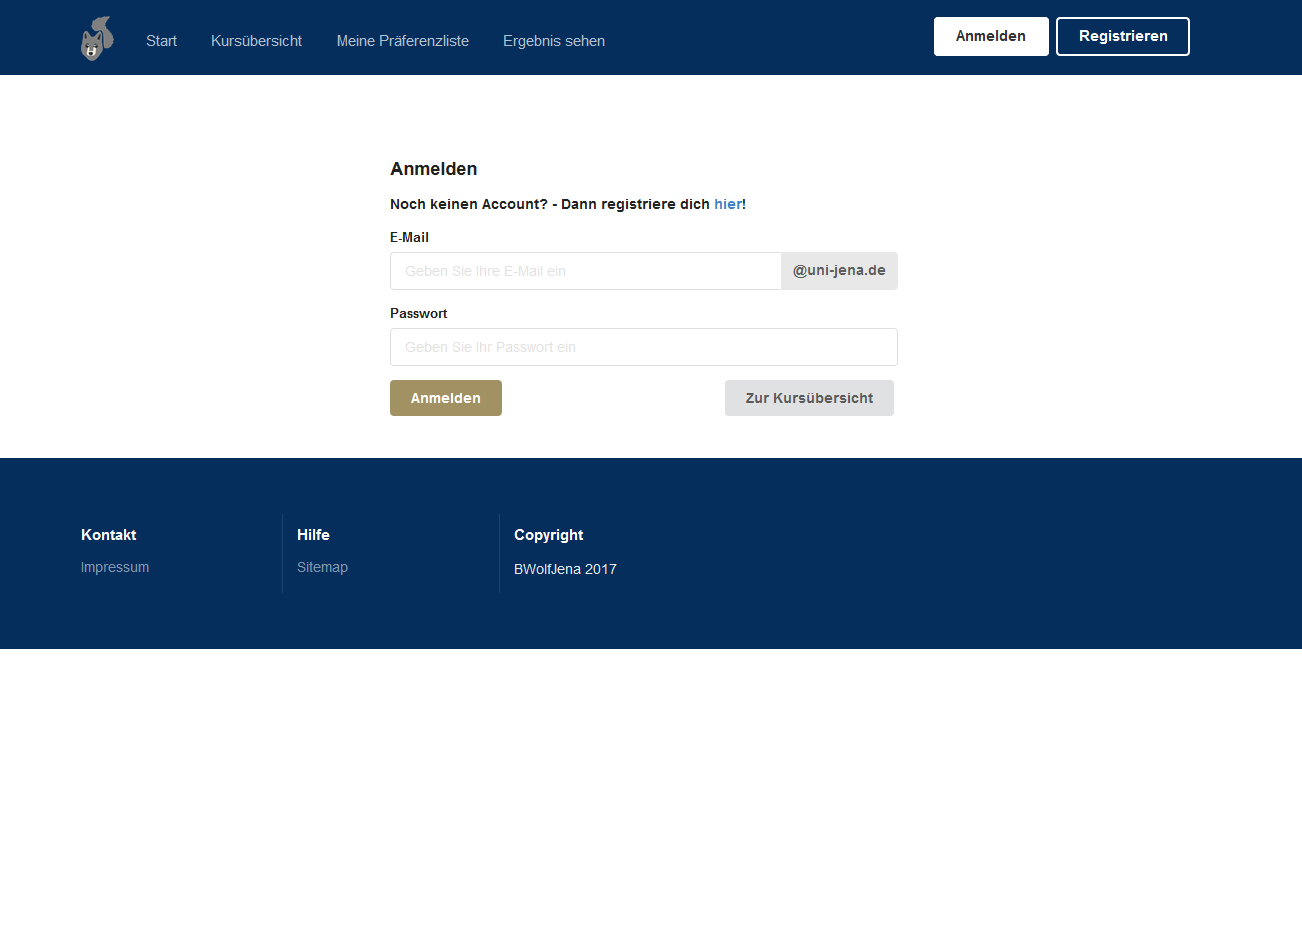
\includegraphics[width=1.0\textwidth]{./implementation/images/login.png}
            \end{subfigure}
            \caption{Gegenüberstellung von Entwurf der Login-Oberfläche (links) und Umsetzung (rechts)}
            \label{fig:comparisonLogin}
        \end{figure}
    
        In Abbildung \ref{fig:comparisonLogin} sind der Entwurf für die Login-Oberfläche und die Umsetzung selbiger gegenüber gestellt.
        Es fällt auf, dass die grobe Struktur der Seite bis auf kleine Änderungen mit dem Entwurf übereinstimmt.
        Unterschiede lassen sich vor allem in der Kopfzeile erkennen.
        So wurde der Reiter \textit{Start} hinzugefügt.
        Anders als zuvor angedacht, fiel die Entscheidung für eine Startseite, in der das Empiriepraktikum kurz vorgestellt wird.
        Des Weiteren wurde der Reiter \textit{Einschreiben} aus Gründen der Verständlichkeit in \textit{Meine Präferenzliste} umbenannt.
        Die Seite erfüllt jedoch die selbe Funktion.
    
        \begin{figure}
            \centering
            \begin{subfigure}{0.49\textwidth}
                \includegraphics[width=1.0\textwidth]{./implementation/images/MockUpsFrontend/frontendCourses.png}
            \end{subfigure}
            \begin{subfigure}{0.49\textwidth}
                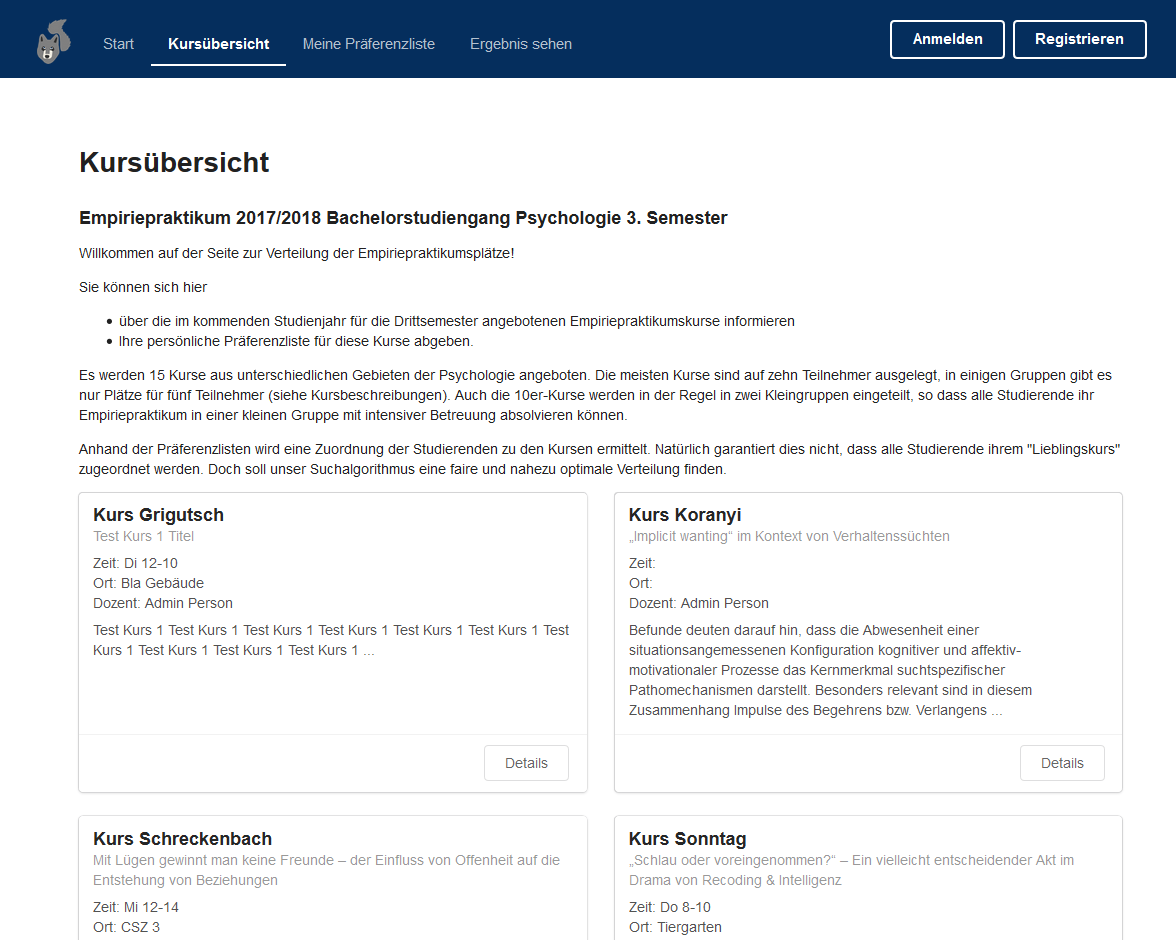
\includegraphics[width=1.0\textwidth]{./implementation/images/courses.png}
            \end{subfigure}
            \caption{Gegenüberstellung von Entwurf der Kursübersicht (links) und Umsetzung (rechts)}
            \label{fig:comparisonCourses}
        \end{figure}
    
        Abbildung \ref{fig:comparisonCourses} zeigt Entwurf und Umsetzung der Kursübersicht.
        Die Struktur des Entwurfs wurde direkt umgesetzt.
        Wie in Kapitel \ref{chapter:requirements} beschrieben, ist es, wie in Abbildung \ref{fig:comparisonCourses} zu sehen ist, möglich auch ohne eine Anmeldung auf die Kursübersicht zuzugreifen.
        Es ist anzumerken, dass die Fußleiste auch in der Kursübersicht wie in Abbildung \ref{fig:comparisonCourses} den Abschluss der Seite bildet und lediglich durch die Menge an Kursen nicht zu sehen ist.
        
        \begin{figure}
            \centering
            \begin{subfigure}{0.49\textwidth}
                \includegraphics[width=1.0\textwidth]{./implementation/images/MockUpsFrontend/frontendPreferences.png}
            \end{subfigure}
            \begin{subfigure}{0.49\textwidth}
                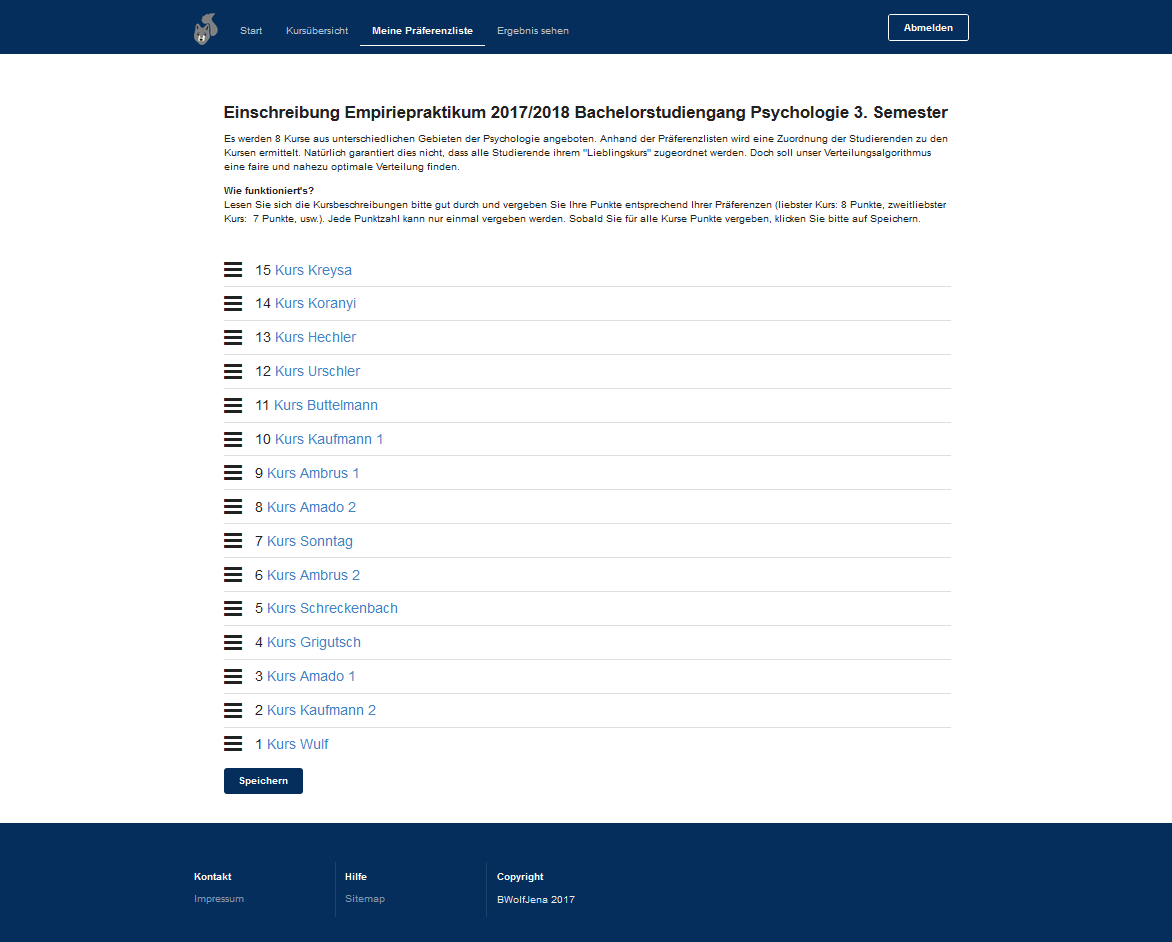
\includegraphics[width=1.0\textwidth]{./implementation/images/preferences.png}
            \end{subfigure}
            \caption{Gegenüberstellung von Entwurf der Einschreibungs-Oberfläche (links) und Umsetzung (rechts)}
            \label{fig:comparisonPrefenrences}
        \end{figure}
    
    
    \section{Backend}
    
        \begin{figure}
            \centering
            \begin{subfigure}{0.49\textwidth}
                \includegraphics[width=1.0\textwidth]{./implementation/images/MockUpsBackend/backendManageCourses.png}
            \end{subfigure}
            \begin{subfigure}{0.49\textwidth}
                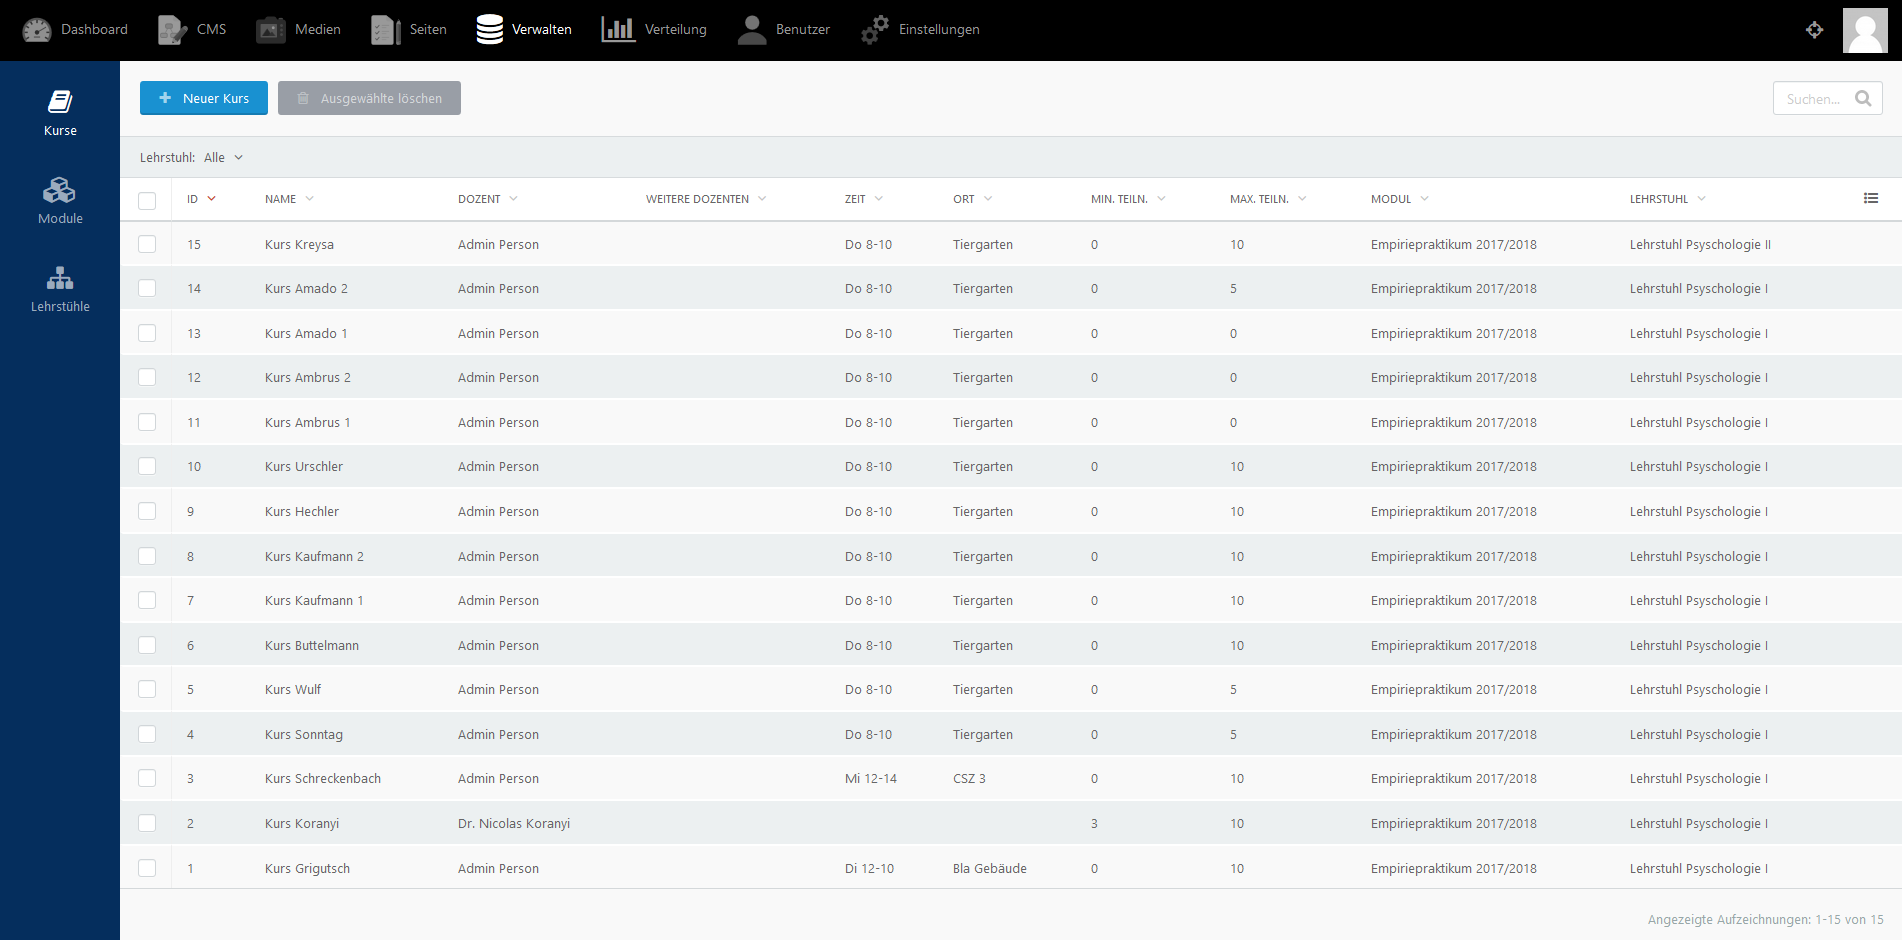
\includegraphics[width=1.0\textwidth]{./implementation/images/manageCourses.png}
            \end{subfigure}
            \caption{Gegenüberstellung von Entwurf der Kursverwaltung (links) und Umsetzung (rechts)}
            \label{fig:comparisonManageCourses}
        \end{figure}
        
        \begin{figure}
            \centering
            \begin{subfigure}{0.49\textwidth}
                \includegraphics[width=1.0\textwidth]{./implementation/images/MockUpsBackend/backendEdit.png}
            \end{subfigure}
            \begin{subfigure}{0.49\textwidth}
                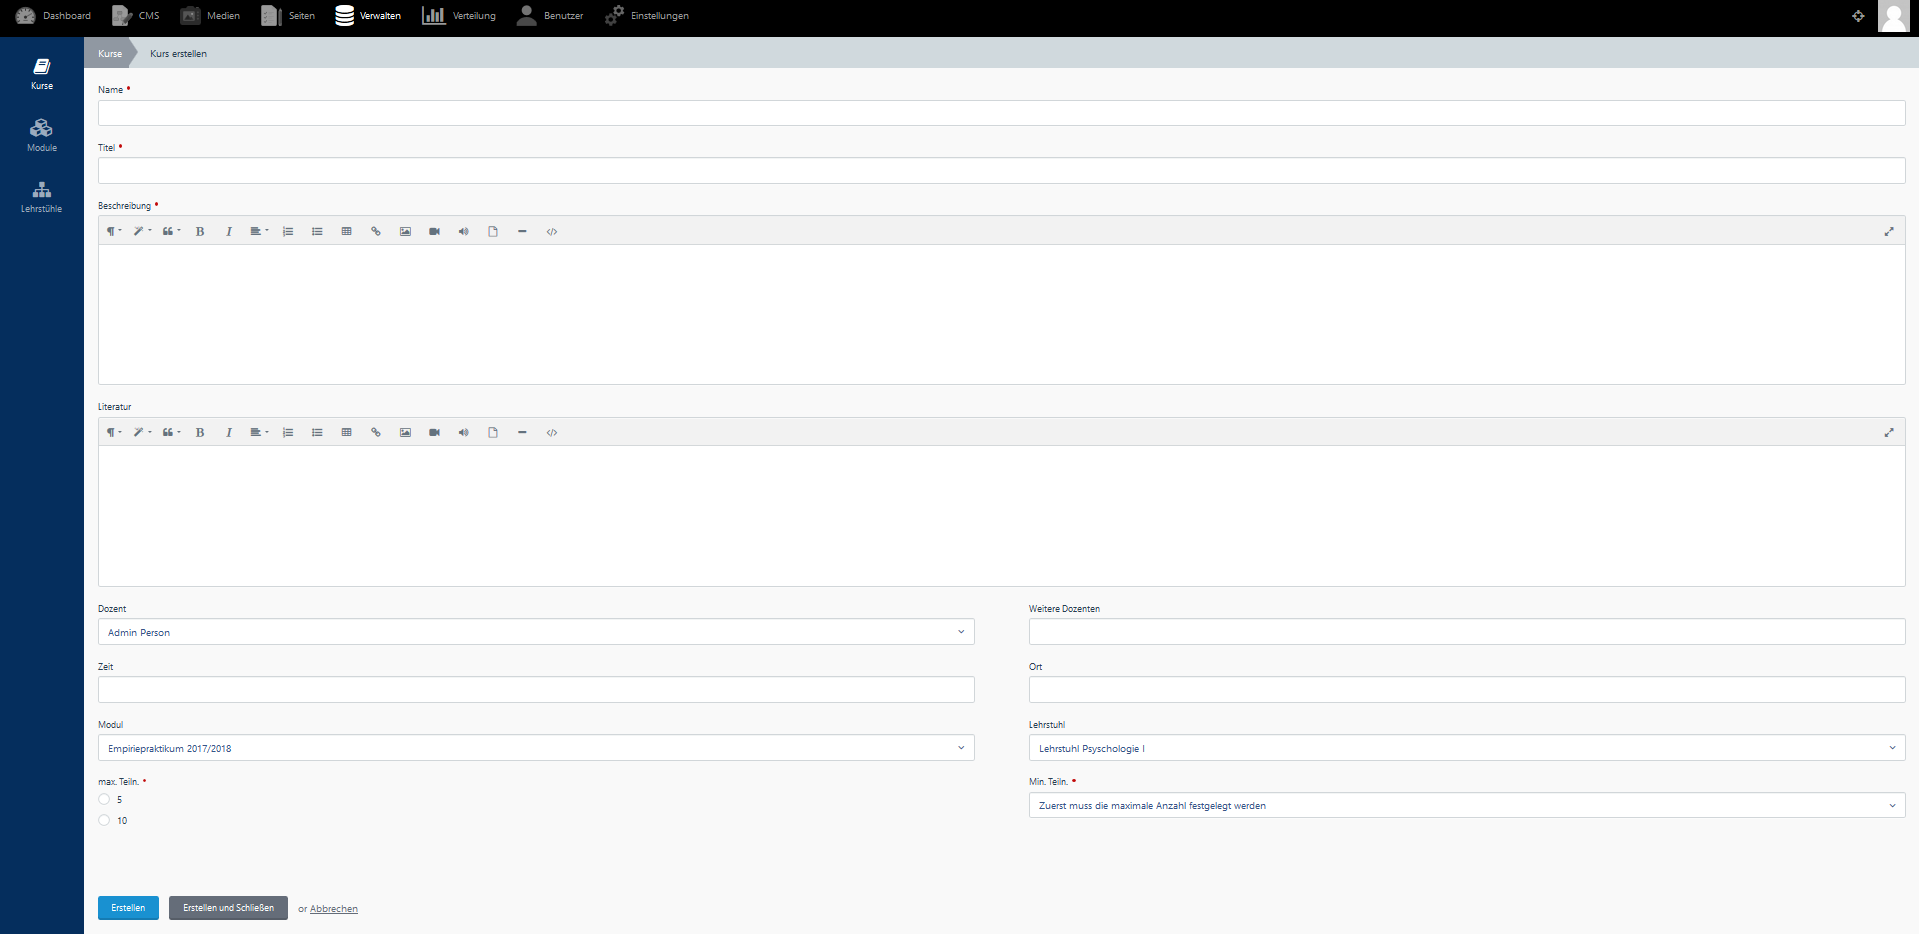
\includegraphics[width=1.0\textwidth]{./implementation/images/edit.png}
            \end{subfigure}
            \caption{Gegenüberstellung von Entwurf der Kurserstellung (links) und Umsetzung (rechts)}
            \label{fig:comparisonEdit}
        \end{figure}
    
        \begin{figure}
            \centering
            \begin{subfigure}{0.49\textwidth}
                \includegraphics[width=1.0\textwidth]{./implementation/images/MockUpsBackend/backendDistribution.png}
            \end{subfigure}
            \begin{subfigure}{0.49\textwidth}
                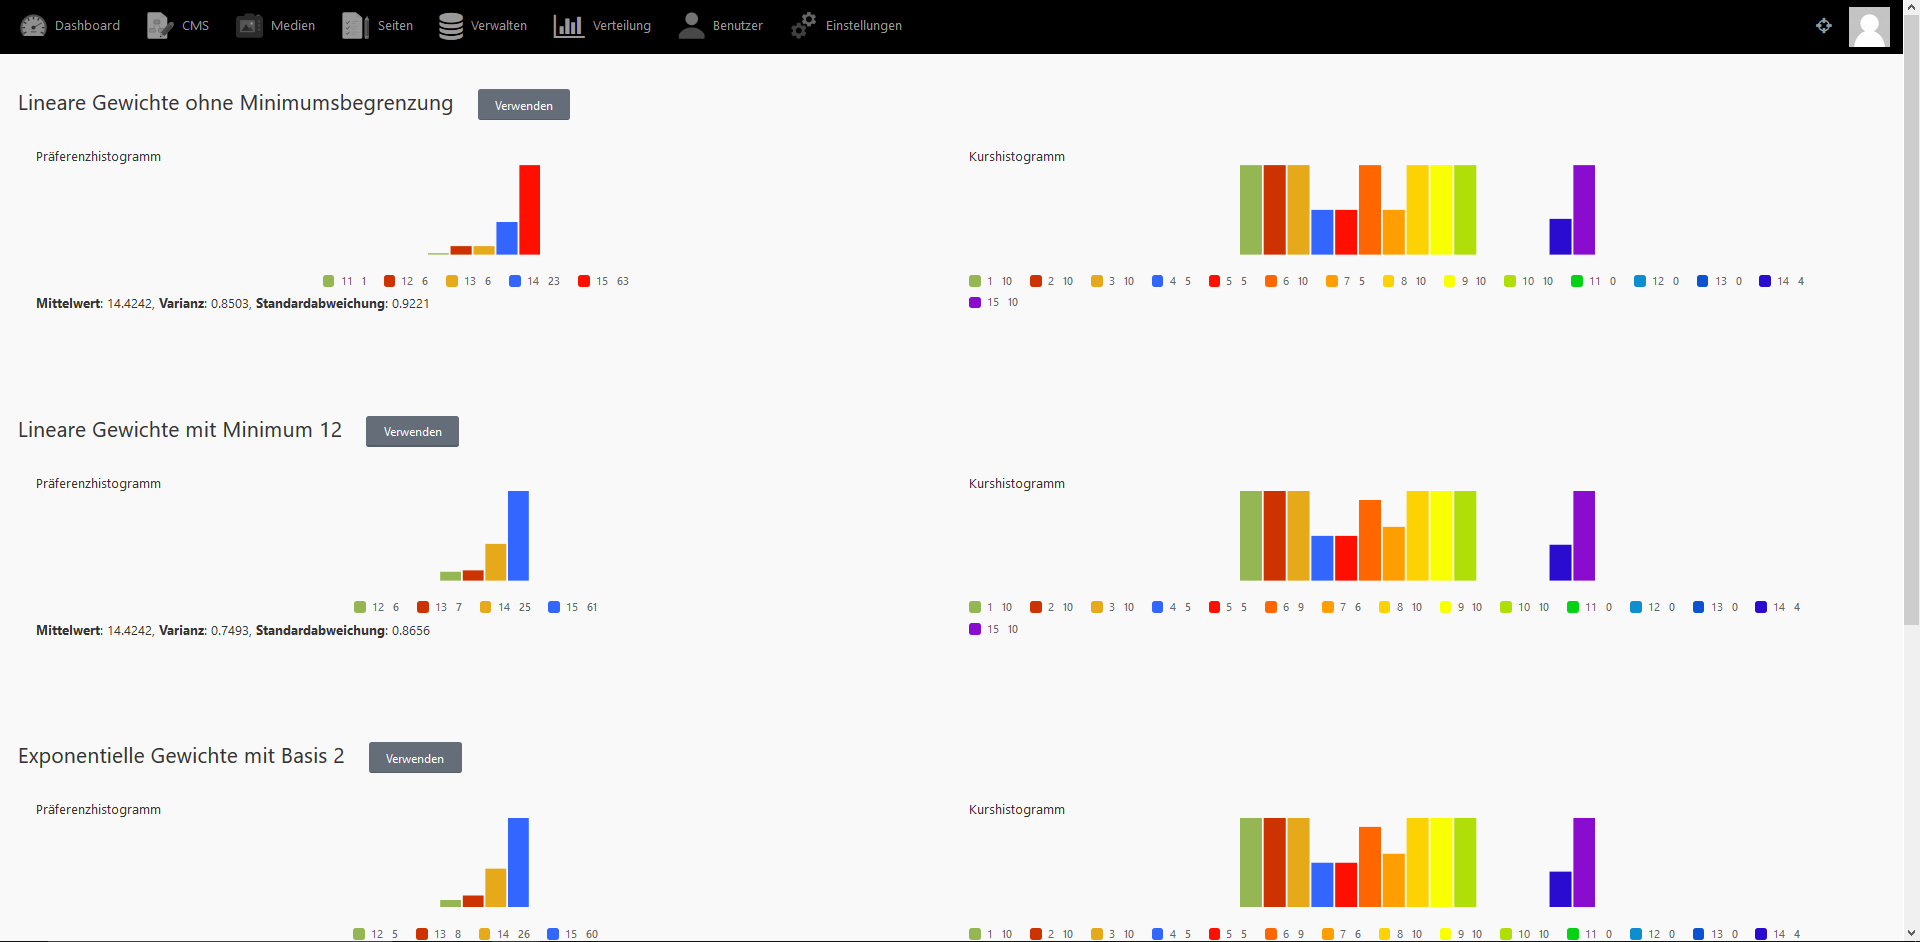
\includegraphics[width=1.0\textwidth]{./implementation/images/distribution.png}
            \end{subfigure}
            \caption{Gegenüberstellung von Entwurf der Anzeige der Verteilungsvorschläge (links) und Umsetzung (rechts)}
            \label{fig:comparisonDistribution}
        \end{figure}
    \section{Überlegungen zum Algorithmus}
        Die Grundlegende Idee der Zielfunktion hat die Form:
            $$ \max ~\text{Summe der Prioritäten} - \text{Gewicht} \cdot \text{Varianz} ~~~.$$
        Genauer ausformuliert ergibt sich:
            $$ \max 
                \sum_{i=1}^{n} \sum_{j=1}^{m} c(i,j)x_{ij} 
                - \frac{\beta}{n} \sum_{i=1}^{n}
                    \left[\left(\sum_{i=1}^{m} c(i,j)x_{ij}\right) - \frac{1}{n} \sum_{i=1}^{n} \sum_{j=1}^{m} c(i,j)x_{ij}\right] ~~~,$$
        wobei gilt:\\
            \begin{tabular}{l c l}
                $n$ & - & Anzahl der Studenten \\
                $m$ & - & Anzahl der Kurse\\
                $ c(i,j) $ & - & Priorität von Student $ i $ für Kurs $ j $\\
                $ \beta $ & - & Gewichtung der Varianz\\
                $t_{\min}(j)$ & - & Minimale Anzahl der Teilnehmer für Kurs $ j $\\
                $t_{\max}(j)$ & - & Maximale Anzahl der Teilnehmer für Kurs $ j $ ~~~.\\
            \end{tabular}\\
        
        Zusätzlich sind drei Nebenbedingungen notwendig, um das Problem angemessen darzustellen.
        Zum einen sollen die $ x_{ij} $ nur die Werte 0 oder 1 annehmen können:
            $$ x_{ij} \in \{0,1\} ~~~.$$
        Des Weiteren soll jeder Student nur einem Kurs zugeteilt werden:
            $$ \forall {i \in \{1,..,n\}}: \sum_{j=1}^{m} x_{ij} = 1 ~~~.$$
        Zuletzt ist die Teilnehmerzahl für die Kurse begrenzt:
            $$ \forall {j \in \{1,..,m\}}: t_{\min}(j) \leq \sum_{i=1}^{n} x_{ij} \leq t_{\max}(j) ~~~.$$
    \chapter{Test des Systems}
\label{chapter:testing}

	Das Testen dieses Softwaresystem wurde in drei Aufgabenbereiche unterteilt.
	Zuerst wurde das Frontend durchgängig getestet.
	Anschließend wurde das Backend überprüft.
	Letztendlich wurde der Algorithmus mit seinen Auswirkungen auf Richtigkeit untersucht.
	
	\section{Frontend}
		Um das Frontend ordnungsgemäß zu testen, muss zuerst die Homepage getestet werden.
		In diesem Fall genügt es, den Header zu testen.
		Dies bedeutet, dass sowohl die Textfelder (''Start'', ''Kursübersicht'', ''Meine Präferenzliste'', ''Ergebnis sehen'') des Headers, als auch die Reihenfolge derer überprüft wird.
		Zusätzlich werden die Texte der Buttons ''Anmelden'' und ''Registrieren'' und die Reihenfolge dieser geprüft.
		Dies geschieht in dem Testfall \textit{HomepageTest}.\newline
		
		Der Testfall \textit{RegisterTest} verifiziert, dass ein Nutzer sich ordnungsgemäß registrieren kann und anschließend auch mit diesen Daten anmelden kann.
		Dafür klickt der automatisierte Nutzer auf den ''Registrieren''-Button der Homepage und registriert sich.
		Anschließend ruft der User die Login-Seite auf und meldet sich an.
		Ein erfolgreicher Login wird durch die Abwesenheit des ''Anmelden''-Buttons sicher gestellt.
		Zu Ende des Testfalls wird der neu registrierte Nutzer gelöscht.
		
		Der darauffolgende Testfall ist \textit{LoginTest}.
		Dieser testet, dass ein bereits registrierter Benutzer sich anmelden kann.
		Dafür wird zuerst ein Nutzer in der Datenbank kreiert.
		Der automatische User öffnet die Login-Seite und gibt die Daten des kreierten Nutzers ein.
		Der erfolgreiche Login wird durch die Abwesenheit des ''Anmelden''-Buttons sicher gestellt.
		Zu Ende des Testfalls wird der kreierte Nutzer aus der Datenbank gelöscht.
					
	\section{Backend}
	
	\section{Algorithmus}
	

    \chapter{Zusammenfassung}
\label{chapter:summary}
Zielsetzung des Projekts war es, eine Plattform zu schaffen, mithilfe das Empiriepraktikum des Instituts für Psychologie verwaltet werden kann.
Hierbei sollte vor allem die Möglichkeit der automatischen Verteilung der Studenten anhand von Präferenzlisten umgesetzt werden.
Diese und weitere Anforderungen wurden im Rahmen dieser Arbeit herausgearbeitet.
Vor allem die Aufteilung in die Verschiedenen Rollen Studenten, Dozenten und Administratoren mit unterschiedlichen Sichten auf das System waren ein wichtiger Anspruch.
Basierend auf diesen Anforderungen wurde ein Entwurf für das System entwickelt und vorgestellt.
Dieser umfasste neben Mockups für die wichtigsten Seiten der Plattform die Aufteilung in ein Front- und Backend mit dazugehörigem Datenmodell.
Anschließend konnte die Umsetzung der Entwürfe erfolgen.
Große Teile wurden dabei mit dem Framework \textit{October CMS} realisiert.
Nachdem der Funktionsrahmen der Plattform geschaffen war, konnte der Verteilungsalgorithmus entwickelt werden.
Eine geeignete lineare Zielfunktion wurde aufgestellt und eine mögliche Wahl der Parameter und weitere Varianten der Zielfunktion diskutiert.\\

Im Anschluss wurden die Tests der Plattform zur Einschreibung und Verwaltung und des Verteilungsalgorithmus betrachtet.
Anhand der Tests konnte gezeigt werden, dass alle Kernfunktionen des Systems wie gewünscht funktionieren.
Der Verteilungsalgorithmus erreichte auf künstlich generierten Datensätzen gute Verteilungen.
Im Vergleich mit dem Algorithmus der alten Lösung, konnten ein deutlich besseres Ergebnis der Verteilung erzielt werden.\\

Es konnten jedoch nicht alle Anforderungen an das System umgesetzt werden.
So wurde die mögliche Tauschbörse nicht implementiert.
Des Weiteren wird die im Datenmodell angelegte Unterstützung für mehrere verschiedene Module zwar im Backend unterstützt, im Frontend ist es jedoch nicht möglich Präferenzlisten für mehre Module parallel zu verwalten.
Auch konnten einige der im Entwurf angedachten Elemente nicht umgesetzt werden, da durch \textit{October CMS} bereits Teile vorgegeben waren.




    %\section{Stand des Projekts}
        
    %\section{Offene Probleme}
    
    %\section{Mögliche weitere Arbeiten}
    \clearpage
\chapter{Anhang}
\label{chapter:appendix}
    \section{Anhang - Entwurf}
        \begin{figure}[t]
            \centering
            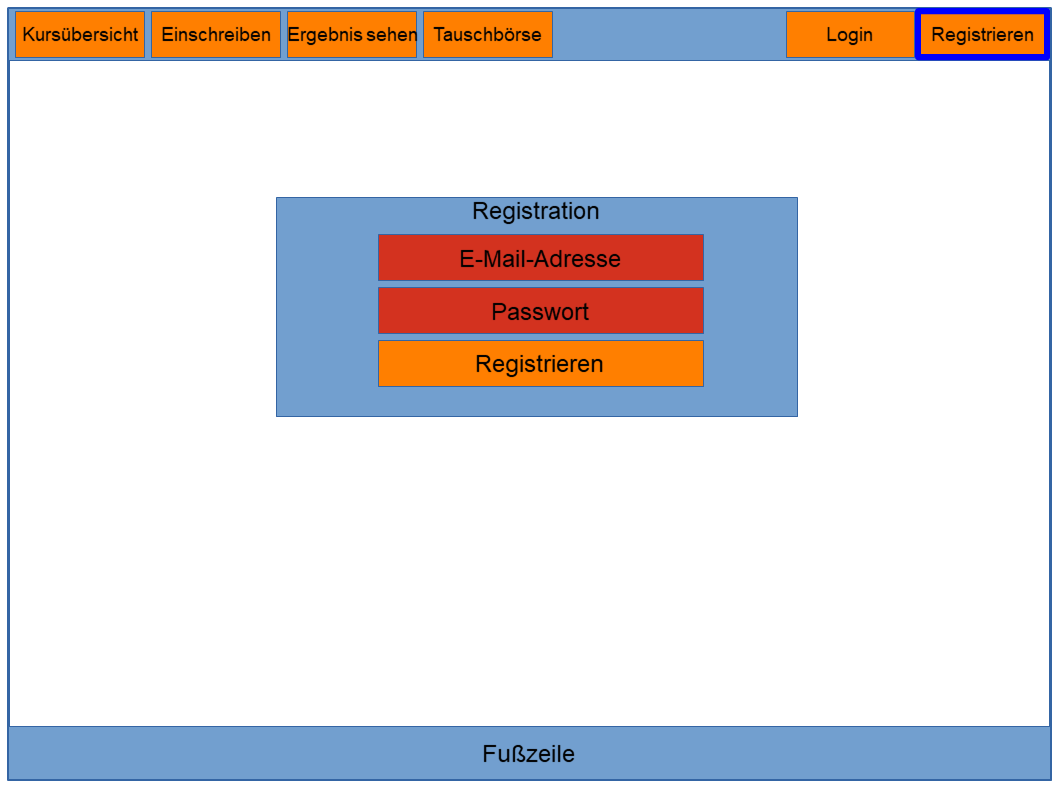
\includegraphics[width=0.7\textwidth]{./design/images/MockUpsFrontend/frontendRegistration.png}
            \caption{Entwurf für Registrierungs-Oberfläche}
            \label{fig:mockupRegistrationFrontend}
        \end{figure}
        
        \begin{figure}[t]
        	\centering
        	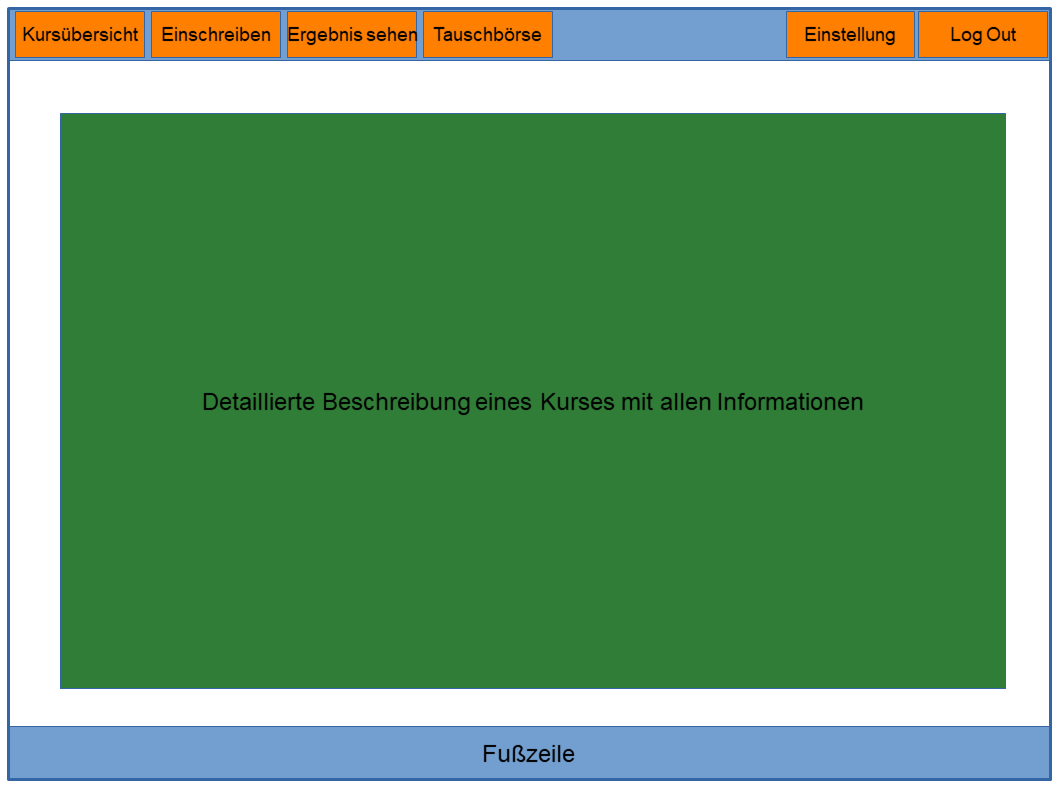
\includegraphics[width=0.7\textwidth]{./design/images/MockUpsFrontend/frontendCoursedetails.png}
        	\caption{Entwurf für die Kursdetails}
        	\label{fig:mockupDetailsFrontend}
        \end{figure}
    
        \begin{figure}[t]
        	\centering
        	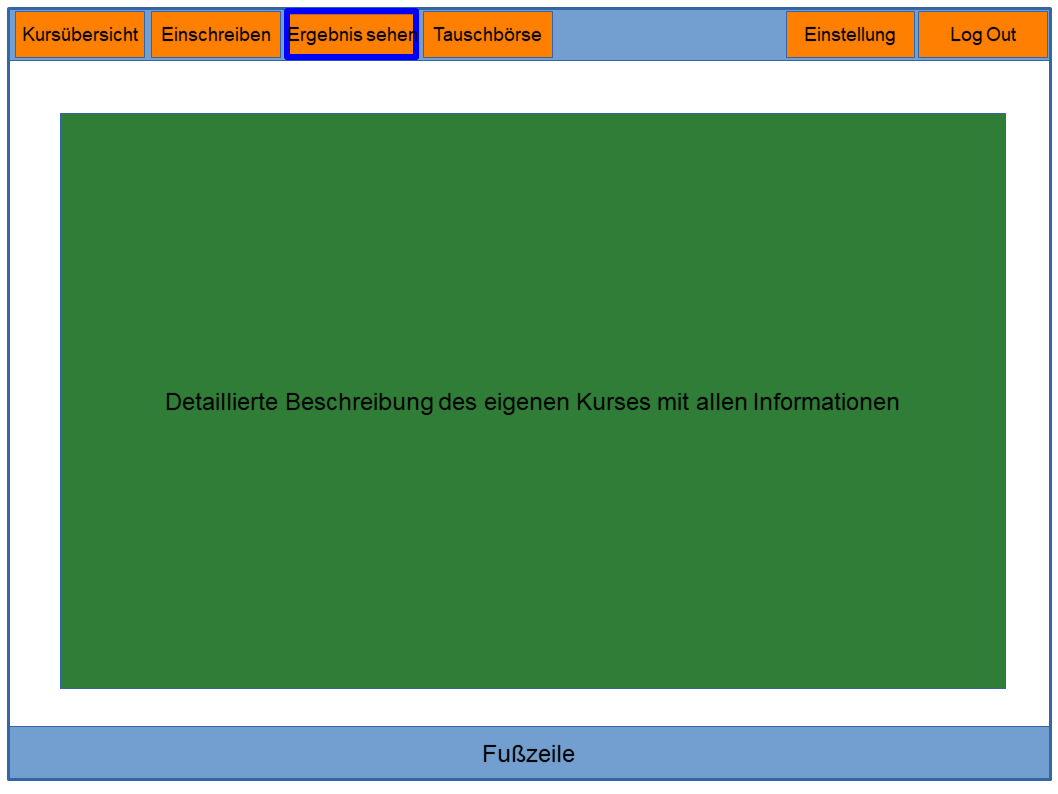
\includegraphics[width=0.7\textwidth]{./design/images/MockUpsFrontend/frontendResults.png}
        	\caption{Entwurf für die Ergebnisübersicht}
        	\label{fig:mockupResultsFrontend}
        \end{figure}
    
        
    
    
    
\end{document}